\section{Conditional probability and Bayes' Theorem} \label{s7} 

\subsection*{\hspace{3.3ex}``A problem in the doctrine of chances''}

\ssn{Learning Outcomes}
After studying this week you will be able to:
\begin{itemize}
\item calculate conditional probabilities and conditional expectations from the definition;
\item use Bayes' Theorem to establish ``probabilities of causes'' and relate $\PP(A \st B)$ to $\PP(B \st A)$;
\item use ``conditioning on an event'' to compute probabilities and expectations in simple examples. 
\end{itemize}
\end{n}

\subsection{Preparation for the week}

\ssn{Motivating questions}
\begin{itemize}
\item I toss a coin 6 times and get a total of four heads. What is the probability my first roll was heads?   
\item I roll a D6 until I roll two `6's in a row. What is the expected number of rolls this takes. 
\item Why do England lose at football? 
\end{itemize}
\end{n}

\ssn{Revision} 
We have previously used conditional probability in an informal way. For instance, the probability of HHHH in four tosses of a coin is $1/16$.  But the probability of HHHH \emph{given that we know that the first toss is H is $1/8$.}   We write 
 \[
  \PP( \text{HHHH} \st \text{first toss is H}) = \frac18. 
 \]
 
We have used the formula that $\PP(A \cap B) = \PP(A)\, \PP(B \st A)$ very often.  I draw two cards at random, without replacement, from a set of ten numbered $1,2,\dots,10$. What is the probability that I draw an odd number followed by an even number?  Let $B$ be the event that the first card is odd, so $\PP(B)=1/2$. Let $A$ be the event that the second card is even.  Given that $B$ has occurred, there are 5 even cards left and 4 odd so 
 \[
    \PP( \text{second card is even} \st \text{first card is odd} 
     =\PP(A \st B) = \frac59.
 \]
Thus the answer to our question is 
 \[
 \PP(A \cap B) = \PP(B) \PP(A \st B) = \frac12 \, \frac59 = \frac5{18}.
 \]
 Note that this is close but not equal to $1/4$ which would be the probability if we had replaced the first card before drawing the second.
 
Often one takes a calculation and turns it round to provide a definition, as we do now.
\end{n}

\ssn{Definition}
Let $A,B$ be events with $\PP(B) \not=0$.  Then the conditional probability of $A$ given $B$ is defined by 
 \[
    \PP( A \st B )    = \frac{\PP(A \cap B)}{\PP(B)}. 
 \]
\end{n}

\ssn{Example}
My friend tosses two D6 in secret and tells me their sum is 8.  What is the probability that one of the dice is a `6'?

Take the sample space to be all 36 possible rolls of two dice. Let $B$ be the event that the sum is 8.  Let $A$ be the event that one of the dice is a `6'.   Then $A \cap B$ corresponds to just the two possible rolls (6,2) and (2,6). So $\PP(A \cap B) = 2/36$.   Also there are five rolls of two D6 that result in a sum of 8, so $\PP(B) = 5/36$.     Thus 
 \[
       \PP( \text{at least one roll is a `6'} \st \text{sum = $8$ } )  =
        \frac{2/36}{5/36} = \frac25.
 \]
\end{n}

\ssn 
I toss a coin 5 times and obtain 3 or more heads.  What is the probability that the first toss was H? 

Let $B$ be the event of 3 or more H out of 5.  Then by binomial 
 \[
     \PP( B) = \frac1{2^5}\left(  \binom53 + \binom54 + \binom55 \right)   =  \frac{16}{2^5}.
 \]
Let $A$ be the event that the first toss is H.  Then $A \cap B$ is the event of tossing a H, followed by at least 2 H in the remaining 4 tosses. So by binomial again 
 \[
   \PP(A \cap B) = \frac12 \; \frac1{2^4} \left(  \binom42 + \binom43 +\binom 44\right) = \frac{11}{2^5}.
 \]
 So dividing, 
  \[
  \PP(A \st B) = \frac{11/2^5}{16/2^5} = \frac{11}{16}.  
 \]

\end{n}

\ssn{``Zooming in''}
In taking probabilities conditional upon an event $B$, one is zooming in on $B$, replacing ones initial sample space $S$ with $B$. In doing so, one becomes interested in $A \cap B$ rather than $A$ itself.  Figure~\ref{condo} illustrates what is going on. 
\end{n}


\begin{figure}[h] \centering
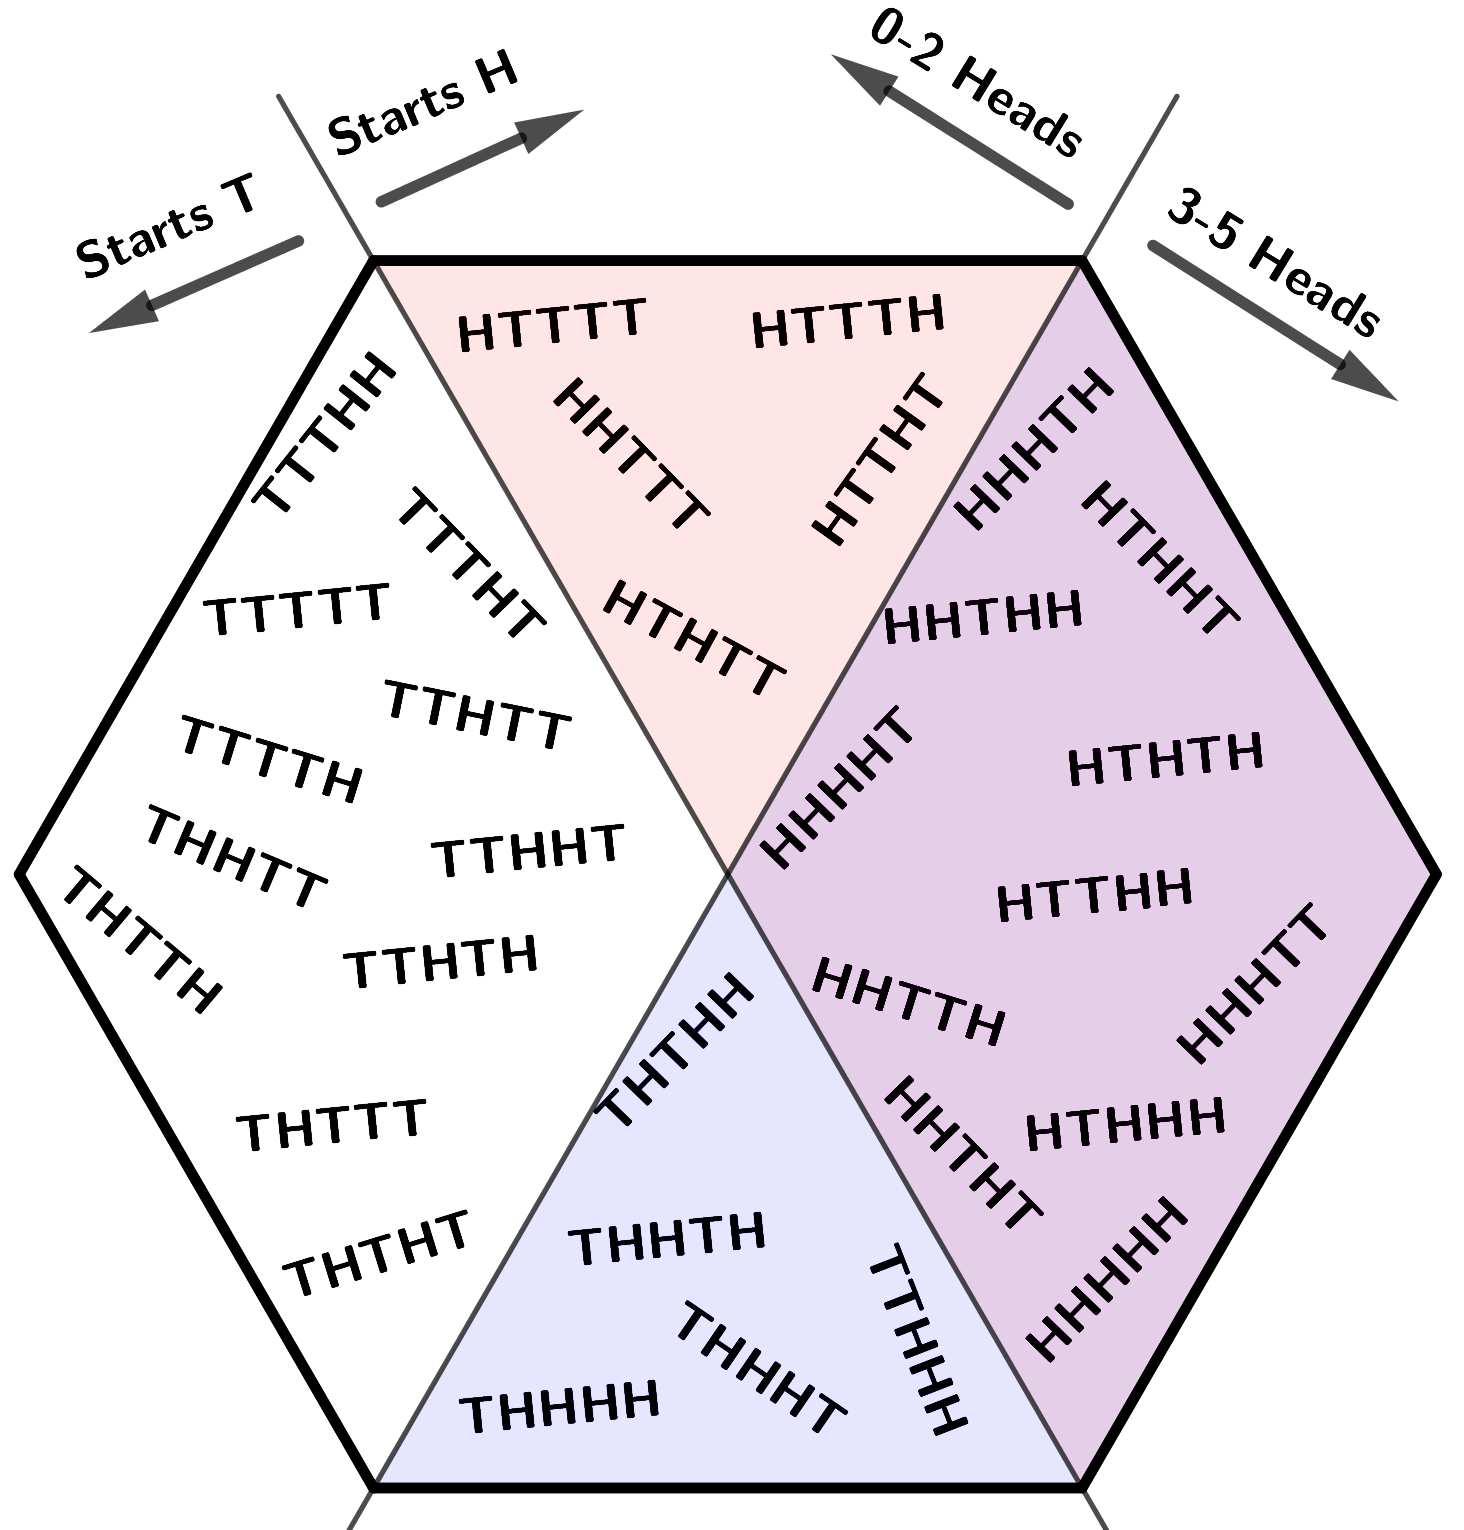
\includegraphics[width=0.52\textwidth]{images/condo0.png}\qquad
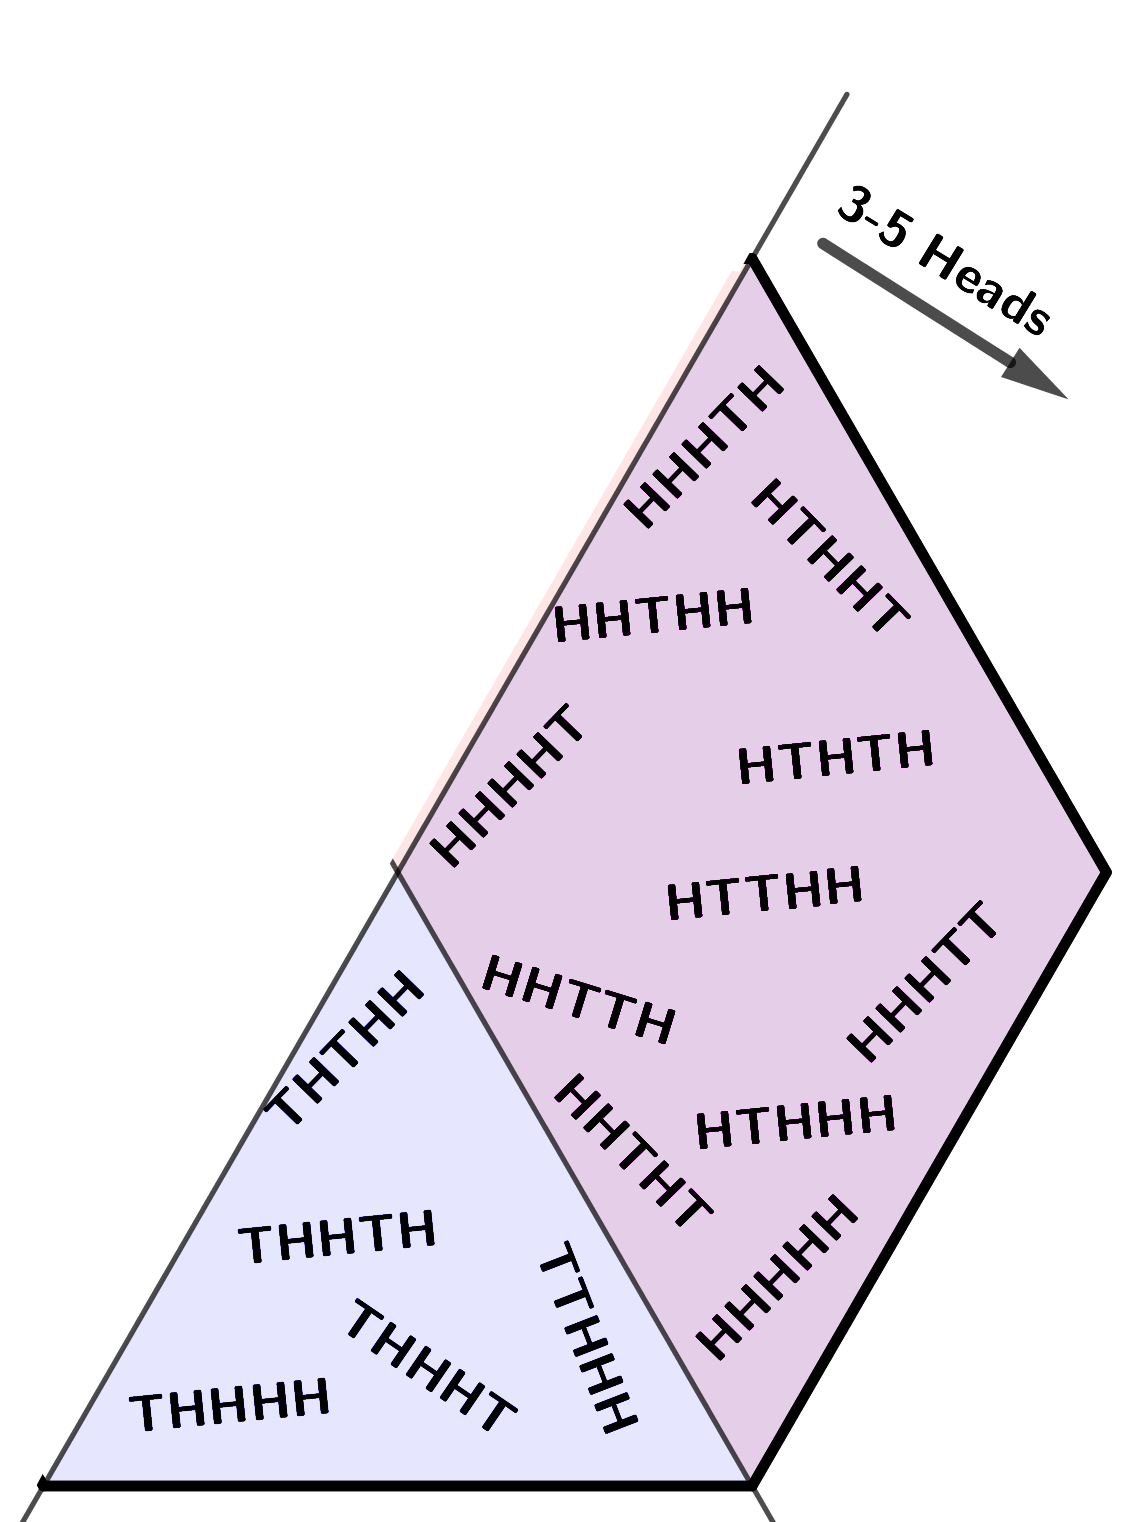
\includegraphics[width=0.4\textwidth]{images/condo1.png}
\caption{\label{condo} The whole sample space for 5 coin tosses (left). ``Zooming in'' on the half with $\geq 3$ heads, we see that $11/16$ start with an `H'. So $\PP(\text{starts with H} \st \text{number of H $\geq 3$ }) = 11/16$.} 
\end{figure}

\ssn{Bayes' Theorem} 
Let $A,B$ be events with $\PP(B)\not= 0$.  Then 
 \[
    \PP( A \st B) = \PP( B \st A) \frac{\PP(A)}{\PP(B)}.
 \]
\begin{proof}
Combine $\PP(A \cap B) = \PP(A \st B) \PP(B)$ with $\PP(A \cap B) = \PP(B \st A) \PP(A)$. 
\end{proof}
\end{n}

\ssn{Bayes' Theorem (``probability of causes'' form) }
Let our sample space $S$ be partitioned into disjoint events $A_k, \, k=1,2,\dots, n$.  Then for $1\leq j \leq n$, 
 \[
   \PP(A_j \st B)  =   \frac{\PP(B \st A_j)\,\PP(A_j)}{ \sum_{k=1}^n \PP(B \st A_k) \,\PP(A_k)}
 \]
\begin{proof}
Put $A=A_j$ in the previous version of the theorem and then expand $\PP(B)$ using the law of total probability (\S\ref{ltp}): 
 \[
   \PP(B) = \PP(B \st A_1) \PP(A_1) + \dots + \PP(B \st A_n) \PP(A_n).
 \]
\end{proof}
\end{n}

\ssn{Example}
The use of the the ``probability of causes'' form is more straightforward than it might appear from the statement. 

Tom and Dick are both liars: independently for everything they say, they tell the truth with probability $1/3$ and lie with probability $2/3$.  Tom says something.  Dick tells me that Tom is telling the truth.  What is the probability that Tom is telling the truth? 


\tikzset{
  treenode/.style = {shape=rectangle, rounded corners,
                     draw, align=center,
                     top color=white, bottom color=blue!30},
  root/.style     = {treenode, font=\Large, bottom color=red!30},
  env/.style      = {treenode},
  branch/.style = {treenode, bottom color=blue!10},  
  dummy/.style    = {circle,draw}
}
\tikzstyle{level 1}=[level distance=4.0cm, sibling distance=3.5cm]
\tikzstyle{level 2}=[level distance=5.0cm, sibling distance=2.0cm]

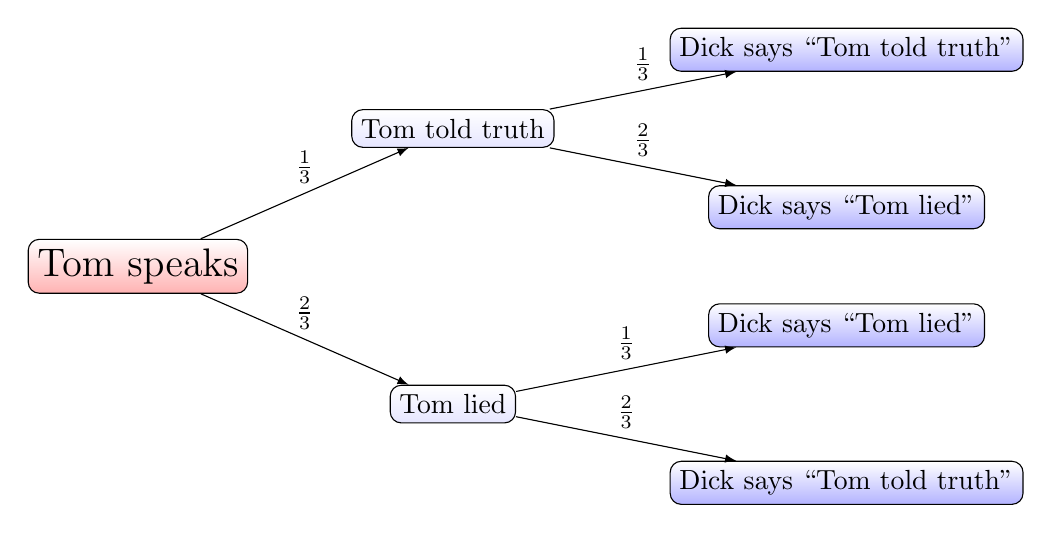
\begin{tikzpicture}
[
grow=right,
    edge from parent/.style = {draw, -latex},
    every node/.style       = {font=\normalsize}
  ]
\node[root]{Tom speaks}
child { 
    node[branch]{Tom lied}
    child { 
        node[env]{Dick says ``Tom told truth''}  
        edge from parent node[above]{$\frac23$} 
        }       
    child { 
        node[env]{Dick says ``Tom lied''}                 
        edge from parent node[above]{$\frac{1}{3}$} 
        }       
    edge from parent node[above]{$\frac23$}            
    }
child { 
    node[branch]{Tom told truth}
    child { 
        node[env]{Dick says ``Tom lied''}                
        edge from parent node[above]{$\frac{2}{3}$} 
        }       
    child { 
        node[env]{Dick says ``Tom told truth''}               
        edge from parent node[above]{$\frac{1}{3}$} 
        }       
    edge from parent node[above]{$\frac{1}{3}$}            
    }     ;           
\end{tikzpicture}

Here, we let $A_1$ be ``Tom told truth'' and let $A_2$ be ``Tom lied''.    We let $B$ be the event that ``Dick says Tom told truth''. 
We are asked to calculate $\PP( A_1 \st B)$. So, using Bayes' theorem in the ``probability of causes'' version we have 
 \begin{eqnarray*}
   \PP( A_1 \st B) &=& 
     \frac{\PP(B \st A_1) \, \PP(A_1)}
     {  \PP(B \st A_1) \,\PP(A_1) + \PP(B \st A_2)\,
         \PP(A_2)   } \\
    &=& \frac{ (1/3)(1/3)}{(1/3)(1/3)+(2/3)(2/3)}  = \frac15. 
 \end{eqnarray*}
\end{n}

\ssn{Example}
The example we will now study is presented as an ``updating information'' example where we use the original Bayes' theorem.  You might like to convert it to a ``probability of causes'' wording and draw the probability tree to understand the connection.

A suspect X is believed to be guilty of a given crime with probability $\PP(G)=0.6$ on the basis of existing evidence.  The criminal also left a blood stain at the scene. The suspect X has a blood group common to 20\% of the general population.

A test on the blood stain now tells us that it comes from a person with this blood group. How does that affect the probability that the suspect X is guilty? 


Let $B$ be the event that the blood stain has this particular blood group.  We know the blood test will certainly be positive if X is guilty, so $\PP( B \st G) = 1$.  But we want to know the probability of X's guilt, given the new evidence. In other words, we want to find $\PP( G \st B)$. 


First we calculate (law of total probability again) 
 \begin{eqnarray*}
  \PP(B) &=& \PP(\text{X guilty}) \,\PP(B \st \text{X guilty})   + \PP(\text{X not guilty}) \,  \PP(B \st \text{X not guilty} ) \\
  &=& (0.6) (1) + (0.4) (0.2)  = 0.68
 \end{eqnarray*}
 because if X is not guilty, the blood test will be positive with the probability of its being so in the general population.
 
Then according to Bayes' Theorem
 \[
    \PP( G \st B) =  \frac{\PP( B \st G)}{\PP(B)} \, \PP(G)
    =  \frac{1}{0.68} \, 0.6 = 0.88 
 \]
is an updated probability of X's guilt. 

Bayes' Theorem has been widely used in court cases. See \url{https://www.theguardian.com/law/2011/oct/02/formula-justice-bayes-theorem-miscarriage} for a controversy a few years ago around this. (Colin Aitken, until recently in the School of Mathematics in Edinburgh is quoted.) 
\end{n}

\sse{}
I toss a coin 6 times and get a total of four heads. What is the probability my first roll was heads?  (Ans: $2/3$.) 
\end{e}

\pagebreak

\subsection{Notes}

\ssn{Conditioning a random variable}
Let $X$ be a discrete random variable and let $B$ be an event with $\PP(B)\not=0$. 
Then the \emph{(conditional) probability that $X=k$ given $B$} is defined as  
 \[
   \PP( X=k \st B ) = \frac{ \PP(\text{$X=k$ and $B$})}{\PP(B)}.
 \]
(In other words, we simply treat $X=k$ as defining an event and use our existing definition.) 
\end{n}

\ssn{Example}
Roll two D6 one after the another. Let $X$ be the sum of the two rolls. Then $\PP(X=8)=5/36$. 
\begin{itemize}
\item Let $B$ be the event that the first roll is a $3$. Then $\PP(X=8 \st B) = 1/6$ since we have to roll 5 on our second roll to achieve $X=8$. 
\item Let $C$ be the event that the first roll is a $1$. Then $\PP(X=8 \st C) = 0$ since it is now impossible. 
\end{itemize}
\end{n}

\ssn{Conditioning expectation}
With that definition in hand, we can define expectations conditioned on an event $B$ for a discrete random variable $X$. 
\[
    \EE( X \st B ) =  \sum_k k \,\PP( X=k \st B). 
\]
\end{n}

\ssn{Example}
We roll two dice again. Let $X$ denote their sum.  We know $\EE(X)=7$. Let $B$ be the event that the first roll is a `2'. 
Then 
 \[
\PP(X=k \st B) = \frac{\PP(\text{$X=k$ and $B$})}{\PP(B)} 
 = \frac16 \quad \text{for $k= 3,\dots,8$ and $0$ otherwise}. 
 \] 
 Then we can calculate $\EE(X \st B) = \sum_k \PP( X=k \st B) \, k = 11/2.$
 
 We could see the answer to this also directly: we have rolled `2' already and the expected value of the second roll is $7/2$ and $2 + 7/2 = 11/2$. 
\end{n}

\ssn{Example}
Let $X$ be the number of rolls of a D6 until we get the first `6'.  This is a geometric random variable with expected value $6$. 

Let $B$ be the event that the first roll is a `3'.  Then $\EE(X \st B) = 7$ because after the first roll, we still have the expected number of rolls until we get a '6' being $6$.  
\end{n}   

\ssn{Example}
I roll a D6. What is the probability $p$ that I get the first `6' before I roll any odd numbers? 

 Let $W$ be the event that I roll a 6' before any odd numbers. 
Let $A$ be the event that my first roll is odd. Let $B$ be the event that my first roll is a `6'.   Let $C$ be the event that my first roll is a `2' or a `4'.  

Then $\PP(W \st A) = 0$ and $\PP(W \st B) = 1$.  On the other hand, rolling a `2'or a `4' has no effect on my likelihood of achieving $W$.   So $\PP(W \st C) = p$. 
So
\begin{eqnarray*}
 p = \PP(W) &=& \PP(W \st A) \PP(A) + \PP(W \st B) \PP(B) + 
 \PP(W \st C) \PP(C) \\
  &=&  0 \,\frac12 + 1 \, \frac16 + p \frac13.
\end{eqnarray*}
Solving, $p=1/4$. 

Several more examples of conditioning on the first step and then doing this ``referring back to the original problem'' trick can be found in lectures. 
\end{n}


\ssn{Theorem (Law of total probability for expectations)}
Let $S = A_1 \cup A_2  \cup \dots \cup A_n$ be a partition of a sample space into $n$ events. Let $X$ be a random variable on $S$.  Then 
 \[
   \EE(X) = \EE(X \st A_1) \, \PP(A_1) + \dots + \EE(X \st A_n) \, \PP(A_n).
 \]
 \begin{proof}
 \begin{eqnarray*}
  \EE(X) &=& \sum_k k\, \PP(X=k) \\
     &=& \sum_k k \left( \sum_j \PP(X=k \st A_j) \, \PP(A_j) \right) \\
    &=& \sum_j 
    \left( \sum_k k \,  \PP(X=k \st A_j) \, \PP(A_j)  \right) \\
   &=& \sum_j \PP(A_j) \left( \sum_k k \,  \PP(X=k \st A_j)  \right) \\
    &=& \sum_j \PP(A_j)  \EE( X \st A_j) 
 \end{eqnarray*}
 \end{proof}
\end{n}

\ssn{Example}
I choose a D3 a D4 or a D6 uniformly randomly and roll it.  What is my expected roll?   

Let $X$ be my final roll. Then 
 \[
  \EE(X) = \EE(X \st D3) \PP(D3) + \EE(X \st D4) \PP(D4) + 
  \EE(X \st D6) \PP(D6)  = \frac13 \, 2 + \frac13 \, \frac52 + \frac13 \, \frac72 = \frac83. 
 \]
\end{n}

\ssn{Example}
 A quick way to calculate the expected value of a geometric RV $X \sim \mathrm{Geom}(p)$.
 
Let $A$ be the event that I succeed on my first trial. Let $m = \EE(X)$. 
Then $\EE(X \st A) = 1$ and $\EE(X \st A^c) = m+1$ because in the first case I have already succeeded and in the second case I have used up one trial and have to start again.  

Then conditioning on $F$ we have 
 \[
  m = \EE(X) = \EE(X \st A) \PP(A) + \EE(X \st A^c ) \PP( A^c) = 
     1 \, p +   (m+1) (1-p) = m+1 - mp.  
 \]
 Solving, $m=1/p$. 
\end{n}


\subsection{Exercises and problems}

\sse 
Evaluate
\begin{enumerate}
\item Let $X$ be the result of rolling a D6. What is the probability of $X=6$ given that $X$ is even?  What is the expected value of $X$ given that $X$ is even? 
\item Rolling a D6, let $Y$ be the number of rolls it takes until I roll a `6'. What is the probability that $Y=5$ given that $Y>3$? 
\item Rolling a D6 again, what is the expected total number of `6's I roll in 8 attempts, given that my first two rolls are 6,2?  
\end{enumerate}
Answers: (1) $1/3$, $4$; (2) $5/36$; (3) $2$.  
\end{e}


\sse 
A very standard example of this sort of ``probability of causes'' analysis is ``false positives'' in medicine. For example, suppose that in the general population, a certain condition is present in 1\% of people.  

There is a test for the condition. The test always returns positive if the subject has the condition.  If the subject does not have the condition, it returns negative 95\% of the time but gives a positive response 5\% of the time.  

A random person takes the test and it returns positive. What is the probability they have the disease? 
\end{e}

\sss 
You may find drawing the tree helps.   In this case, let $C$ denote the event that the random person has the condition.  Let $T$ denote the event of a positive test result.  From the question 
 \[  
    \PP(C) = 0.01, \quad \PP(C^c) = 0.99, \quad \PP(T \st C) = 1, 
    \quad \PP( T \st C^c)=0.05
 \] 
 where the complement $C^c$ is the event of the person not having the condition. Finally, 
 \[
 \PP(T) = \PP(T \st C) \PP(C) + \PP(T \st C^c) \PP(C^c) = 
   1 (0.01) + 0.05 ( 0.99) = 0.0496.
 \]
We are asked for $\PP( C \st T)$ and so by Bayes,
\[
   \PP(C \st T) = \PP(T \st C) \,\frac{\PP(C)}{\PP(T)} 
   = 1 \; \frac{0.01}{0.0496} = 0.2016. 
\]
(One sees here a basic problem with ``screening'' programmes: unless the test is very reliable, they will throw up many more false alarms than real ones.) 
\end{s}



\sse 
This sort of information updating with Bayes' Theorem is also an essential ingredient in machine learning. It goes something like this. 

Suppose an image identifying algorithm is trying to decide what sort of animal is appearing in a picture on the web.  The word ``cat'' appears in nearby text so the algorithm's initial hypothesis is it's a cat with probability $0.8$. The algorithm decides that there is a ball of string in the picture. It is known that this is the case for 50\% of cat pictures but also for 10\% of non-cat pictures.  What is the updated probability that the picture shows a cat? 
\end{e}

\sss
Here $P(C)0.8$, where $C$ is the event of the picture being of a cat. The probability of a ball of string in the picture is 
 \[
   \PP(S) = \PP(S \st C) \PP(C) + \PP(S \st C^c) \PP(C^c) = 
    0.5 * 0.8 + 0.1 * 0.2 = 0.42,  
 \]
(where $C^c$ is the complement of $C$, i.e.\ the even of the picture not being of a cat).   So, by Bayes: 
 \[
   \PP(C \st S) = \frac{\PP(S \st C)}{\PP(S)} \,\PP(C) =
       \frac{0.5}{0.42} 0.8 = 0.95.
 \]
\end{s}

\ssp 
Tom, Dick and Harry each tell the truth independently with probability $1/3$ and lie with probability $1/3$ every time they speak. Tom says something we don't hear; Dick states whether Tom told the truth or not, but we don't hear that either. Harry says that Dick says that Tom told the truth.  What is the probability that Tom told the truth? 
\end{e}

\sss
From a tree, I compute that Harry says that Dick says that Tom told the truth (``HSDSTTT") with probability $13/27$. Also, the conditional probability that Harry says this given that Tom told the truth (``TTT'') is $5/9$. From Bayes (or just analysing the tree),
 \[
   \PP(TTT \st HSDSTTT ) = \PP( HSDSTTT \st TTT) \frac{\PP(TTT)}{\PP(HSDSTTT)} = \frac59 \, \frac{1/3}{13/27} = \frac5{13}. 
 \]
\end{s}

\sse 

(Optional: why England are poor at football) In football, to oversimplify, if you have possession of the ball close to your own goal you can kick the ball a long way towards the opponents goal and all run after it (the ``long ball game'' (L)), or you can can try to work the ball slowly up the pitch by passing to nearby team mates (the passing game (P)).   It seems England (and other UK teams) have relied too much on the (L) rather than (P) strategy.  

In the 1950s, in an early attempt to apply statistics to sport, data was gathered by Charles Reep live at football matches. The data on the strategy used and whether or not a goal resulted, may have looked something like this\footnote{I don't know if the original data is available, but it would be interesting to find it.}. 

\begin{figure}[h!] \centering 
\begin{tabular}{|ccc|c|}
\hline  
\textbf{Strategy}  & \textbf{Goal (G)}&\textbf{No goal (N)}& \textbf{Total} \\
Long Ball (L) &  30 &  320  & 350 \\
Passing (P) & 20 & 180 &  200 \\
\hline \textbf{Total} & 50  & 500 & 550 \\
\hline 
\end{tabular}
\end{figure}

Suppose we take the ratios in these figures as exactly representing probabilities so that, for instance the probability of a goal is $\PP(G) = 50/550 \approx 1/11$.  Compute also $\PP(L)$, $\PP(L \st G)$ and $\PP(P \st G)$. 

Because $\PP(L \st G) > \PP( P \st G)$, Reep advocated the $L$ strategy.  What is the problem with that reasoning? 

See \url{https://goo.gl/izsafS} for more details and discussion. 
\end{e}

\sss
The probabilities are $\PP(L) = 7/11$, $\PP(L \st G)= 3/5$ and $\PP(P \st G)=2/5$. 

The problem with Reep's reasoning is that he was only seeing more L,G combinations than P,G ones because there was more L than P going on.  The important point as far as deciding whether L or P is superior is which is more likely to lead to a goal.  In other words, he should have considered $\PP(G \st P)$ compared to $\PP(G \st L)$.  From the (invented) data, 
\[ 
\PP(G \st P) = \frac1{10} \quad \text{ and } \quad \PP(G \st L) = \frac3{35}. 
\]
and so the P strategy is more likely to lead to a goal. 
\end{s}

